\begin{figure}
    \centering
    \setlength{\imagewidth}{120mm}%
	\setlength{\imageheight}{0.75\imagewidth}%
	%
	\colorlet{colorRight}{mycolor_2!70!black}
	\colorlet{colorLeft}{mycolor_3!85!black}
	\colorlet{colorPseudoEdS}{mycolor_4!80!black}
	\colorlet{colorAngle}{yellow!20!white}%mycolor_5!12!white}
	%
	\DTLsetseparator{,}%
	\DTLloaddb[noheader,keys={x,y}]{dbisoupoints}{figures/data/pseudo_EdS_arete/iso-u_points.dat}%
    \begin{tikzpicture}[
    	x=\imagewidth,
		y=\imageheight,
		curve/.style = {thick, line cap = round},
		point/.style = {circle, scale=0.27, fill=black},
		vector/.style = {-latex', thick},
		label/.style = {inner sep=2pt},
		txt/.style = {font=\small},
		insert node/.style args={#1 at #2}{
    		postaction=decorate,
    		decoration={
      			markings,
      			mark= at position #2 with {#1}
      		}
		}
    ]
    	%
    	\node[anchor=south west, inner sep=0] {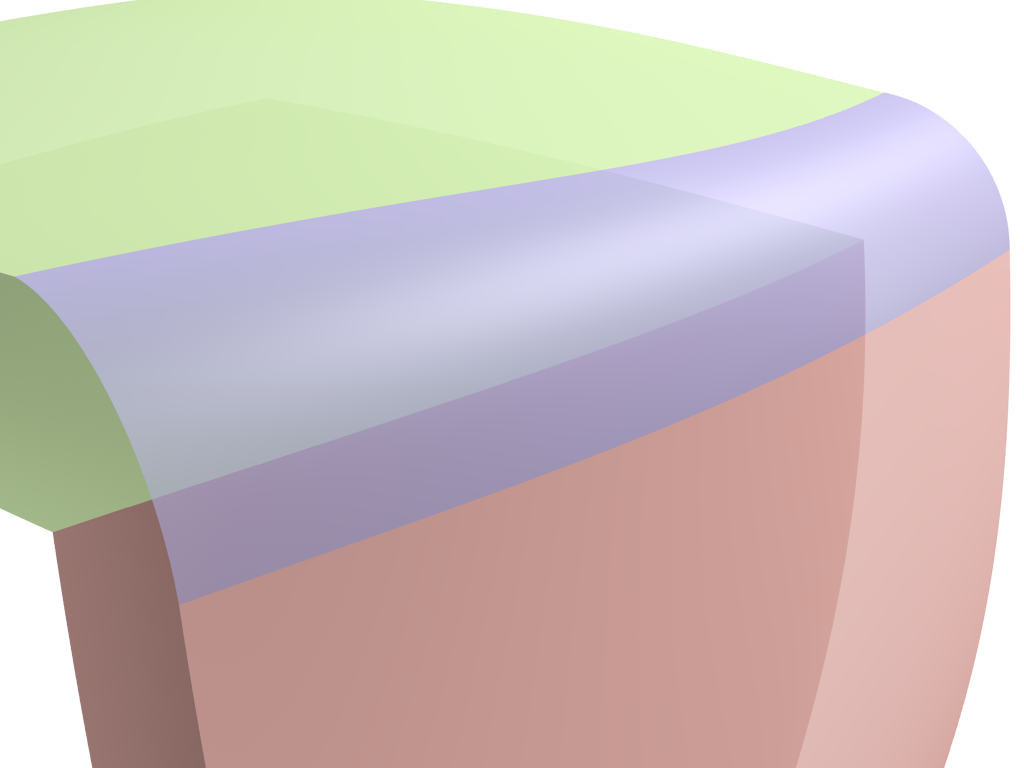
\includegraphics[width=\imagewidth]{pseudo_EdS_arete/pseudo_EdS_arete0001.png}};
    	%
    	{\transparent{0.6}%
    		\draw[curve, dash pattern=on 3pt off 4pt] plot file {figures/data/pseudo_EdS_arete/edge_hidden.dat};
    	}%
    	\draw[
    		curve,
    		insert node={\node[txt, above] {$\brepedge$};} at 0.2
    	] plot file {figures/data/pseudo_EdS_arete/edge_visible.dat};
    	%
    	% iso-v curves (boundary curves)
    	\draw[curve, colorRight] plot file {figures/data/pseudo_EdS_arete/iso-v_curve_0.dat};
    	\draw[curve, colorLeft!90!black] plot file {figures/data/pseudo_EdS_arete/iso-v_curve_1.dat};
    	%
    	% iso-u curve
    	\draw[curve, colorPseudoEdS] plot file {figures/data/pseudo_EdS_arete/iso-u_curve.dat};
    	%
		% points on iso-u curve
		\DTLassign{dbisoupoints}{1}{\ex=x, \ey=y}%
		\coordinate (e) at (\ex, \ey);
		\node[txt, right, colorPseudoEdS!70!black] at (e) {$\eos(u,v)$};
		%
		\DTLassign{dbisoupoints}{2}{\eRx=x, \eRy=y}%
		\coordinate (eR) at (\eRx, \eRy);
		\node[txt, below, colorRight!70!black] at (eR) {$\Right{\eos}(u)$};
		%
		\DTLassign{dbisoupoints}{3}{\eLx=x, \eLy=y}%
		\coordinate (eL) at (\eLx, \eLy);
		\node[txt, above left, inner sep=1pt, colorLeft!70!black] at (eL) {$\Left{\eos}(u)$};
		%
%		\DTLassign{dbisoupoints}{4}{\enx=x, \eny=y}%
%		\coordinate (en) at (\enx, \eny);
%		\draw[vector] (e) -- (en) node[txt, left, inner sep=1pt] {$\unv_{\envelope}(u,v)$};
		%
		\DTLassign{dbisoupoints}{5}{\occx=x, \occy=y}%
		\coordinate (occ) at (\occx, \occy);
		\node[txt, above left, inner sep=0, colorPseudoEdS!90!black] at (occ) {$\bo(u)$};
		\draw[dotted, thick, colorPseudoEdS] (occ) -- (e);
		\draw[dotted, thick, colorRight] (occ) -- (eR);
		\draw[dotted, thick, colorLeft!80!black] (occ) -- (eL);
		%
		\DTLassign{dbisoupoints}{6}{\gx=x, \gy=y}%
		\coordinate (g) at (\gx, \gy);
		\node[txt, below] at (g) {$\bg(u)$};
		%
		\DTLassign{dbisoupoints}{7}{\tx=x, \ty=y}%
		\coordinate (t) at (\tx, \ty);
		\draw[vector] (g) -- (t) node[txt, below right, inner sep=0, shift={(-2pt,-1pt)}] {$\bt(u)$};
		%
		\DTLassign{dbisoupoints}{8}{\rx=x, \ry=y}%
		\coordinate (r) at (\rx, \ry);
		\draw[vector, colorPseudoEdS] (e) -- (r) node[txt, right, inner sep=1pt] {$\br(u,v)$};
		%
		\DTLassign{dbisoupoints}{9}{\rRx=x, \rRy=y}%
		\coordinate (rR) at (\rRx, \rRy);
		\draw[vector, colorRight] (eR) -- (rR) node[txt, right, inner sep=1pt] {$\Right{\br}(u)$};
		%
		\DTLassign{dbisoupoints}{10}{\rLx=x, \rLy=y}%
		\coordinate (rL) at (\rLx, \rLy);
		\draw[vector, colorLeft] (eL) -- (rL) node[txt, right] {$\Left{\br}(u)$};
		%
		\node[txt, colorRight] at (0.92,0.38) {$\EdSpropreplus{\Right{\brepface}}{\rho}$};
		\node[txt, colorLeft] at (0.6,0.9) {$\EdSpropreplus{\Left{\brepface}}{\rho}$};
		\node[txt, colorPseudoEdS] at (0.9,0.75) {$\pseudoEdS{\brepedge}{\rho}$};
		%
		\node[txt, colorRight!50!black] at (0.13,0.15) {$\Right{\brepface}$};
		\node[txt, colorLeft!50!black] at (0.055,0.47) {$\Left{\brepface}$};
		%
		%
		\node[point, colorPseudoEdS!70!black] at (e) {};
		\node[point, colorRight!70!black] at (eR) {};
		\node[point, colorLeft!70!black] at (eL) {};
		\node[point, colorPseudoEdS!90!black] at (occ) {};
		\node[point] at (g) {};
		%
		% angle anotation
		\draw[
			colorAngle,
			insert node={\node[txt, right] {$\theta(u)$};} at 0.68,
			curve, 
			-{Triangle[length=4pt, width=4pt]}, 
			line width=0.6pt, 
		] plot file {figures/data/pseudo_EdS_arete/angle_anotation.dat};
		%
		%
		%\drawGrid{10}{10}{thin, dotted}
	\end{tikzpicture}
    \DTLgdeletedb{dbisoupoints}%
    \caption{Paramétrisation de la pseudo-EdS d'une arête \brep\ convexe.}%$\pseudoEdS{\brepedge}{\rho}$}
    \label{fig:pseudo-EdS_arete}
\end{figure}